% 3DV 2025 / CVPR-style course report: Feedforward 4D Gaussians for Egocentric Vision
\documentclass[10pt,twocolumn,letterpaper]{article}

\usepackage{cvpr}              % camera-ready style (no review ruler)

\input{preamble}

\definecolor{cvprblue}{rgb}{0.21,0.49,0.74}
\usepackage[pagebackref,breaklinks,colorlinks,citecolor=cvprblue]{hyperref}

\usepackage{graphicx}
\usepackage{booktabs}
\usepackage{amsmath}
\usepackage{amssymb}
\usepackage[capitalize]{cleveref}

\def\paperID{FS26}
\def\confName{3DV\xspace}
\def\confYear{2026\xspace}

\title{Feedforward 4D Gaussians for Egocentric Vision}

\author{%
{\setlength{\tabcolsep}{1.2em}%
\begin{tabular}{ccc}
Marian Schneider & Dario Monopoli & Batuhan Iliev \\
{\small Matriculation No: 24-963-118} & {\small Matriculation No: 21-717-632} & {\small Matriculation No: 23-717-457} \\
{\tt\small smarian@ethz.ch} & {\tt\small dmonopoli@ethz.ch} & {\tt\small miliev@ethz.ch} \\
\end{tabular}}\\[0.9em]
ETH Z\"urich, R\"amistrasse 101, 8092 Z\"urich
}

\begin{document}
\maketitle

\begin{abstract}
While 3D Gaussian Splatting (3DGS) has become the standard for real-time radiance
field rendering, extending these models to dynamic, egocentric environments in a
feedforward manner remains challenging. Current 4DGS methods rely on per-scene
optimization and do not exploit egocentric cues such as hand-object interactions.
We extend NeoVerse, a feedforward 4DGS model, with a HaMeR-style head that
estimates a parametric hand model (MANO), and inject its features into the
Gaussian head to guide and supervise the reconstruction. The model jointly
estimates camera poses, hand poses, and pixel-aligned Gaussians. On the HOT3D dataset, hand-feature injection
improves full-frame Gaussian PSNR from $36.96$ to $37.92$ dB over a finetuned
NeoVerse baseline. Our hand head reaches $5.71$ mm PA-MPJPE, down from $5.93$ mm
without local-global fusion. These scene metrics are computed over the full frame
and understate the hand-region gain. We release our training and evaluation code.
\end{abstract}

%==============================================================
\section{Introduction}
\label{sec:intro}

3D Gaussian Splatting (3DGS)~\cite{kerbl20233d} has become a standard explicit
scene representation for high-quality 3D reconstruction. It models scenes as 3D
Gaussians optimized by differentiable rendering. It reaches the quality of
implicit approaches such as Neural Radiance Fields (NeRF)~\cite{mildenhall2020nerf}
while training efficiently and rendering in real time. Feedforward 3DGS
methods~\cite{charatan2024pixelsplat} avoid per-scene optimization and estimate
the Gaussians directly from input images. 4D Gaussian Splatting
(4DGS)~\cite{wu20244d} extends 3DGS to dynamic scenes with a temporal dimension.
Recent geometry foundation models such as DUSt3R~\cite{wang2024dust3r} and
VGGT~\cite{wang2025vggt} predict pose, depth and dense geometry from raw video in
one pass. NeoVerse~\cite{yang2026neoverse} builds on a VGGT backbone and emits a
4D Gaussian field from monocular video.

At the same time, egocentric video has gained increasing attention through
large-scale datasets such as Ego4D~\cite{grauman2022ego4d} and capturing devices
like Project Aria~\cite{engel2023projectaria}. Egocentric data poses specific
challenges. The hands are prominent in the frame, articulate quickly,
self-occlude, and interact with objects. A hand-agnostic 4D world model does not
represent this structure and reconstructs the hand region worst.

The combination of feedforward 4DGS and egocentric data is largely unexplored,
and current pipelines do not use cues such as hand pose. We ask: does an explicit
hand prior injected into a feedforward 4D world model improve egocentric scene
reconstruction, and by how much? We integrate a
HaMeR-style~\cite{pavlakos2024hamer} head that predicts
MANO~\cite{romero2017mano} parameters into NeoVerse, inject its features into the
Gaussian head, and measure the change on HOT3D~\cite{banerjee2024hot3d}.

Our contributions are:
\begin{itemize}
  \itemsep0.15em
  \item We integrate a HaMeR-style MANO hand head into the NeoVerse 4D Gaussian
  model and inject its features into the Gaussian head.
  \item We show that this hand prior improves full-frame scene reconstruction on
  HOT3D. PSNR rises by $0.96$ dB and LPIPS drops from $0.005$ to $0.004$ over a
  finetuned baseline.
  \item We find that local-global fusion between hand crops and scene features
  drives hand accuracy. It lowers PA-MPJPE from $5.93$ to $5.71$ mm, and a variant
  that detaches the hand from the scene gradient is worse on all four metrics.
  \item We report full-frame scene metrics and explain why region-masked
  evaluation is needed to measure the hand-region effect (\cref{sec:discuss}).
\end{itemize}

%==============================================================
\section{Related Work}
\label{sec:related}

\paragraph{Feedforward and dynamic Gaussian Splatting.}
3DGS~\cite{kerbl20233d} and its dynamic extension 4DGS~\cite{wu20244d} achieve
high fidelity but require per-scene optimization. Feedforward methods such as
pixelSplat~\cite{charatan2024pixelsplat} amortize this by predicting
pixel-aligned Gaussians directly, trading per-scene tuning for a learned prior.
We build on this feedforward setting through NeoVerse and study what a
hand-specific prior adds.

\paragraph{Geometry foundation models and 4D world models.}
DUSt3R~\cite{wang2024dust3r} reframed two-view geometry as direct pointmap
regression, and VGGT~\cite{wang2025vggt} scaled this to a transformer that
predicts cameras, depth and tracks jointly. NeoVerse~\cite{yang2026neoverse}
uses a VGGT backbone to produce a 4D Gaussian world model from monocular video.
These models are general and have no notion of hands. We keep the backbone frozen
and add a hand head and a feature-level prior instead of retraining it.

\paragraph{Monocular hand reconstruction.}
The MANO model~\cite{romero2017mano} provides a differentiable, low-dimensional
parameterization of hand pose and shape that is the de facto target for hand
estimation. HaMeR~\cite{pavlakos2024hamer} showed that a plain transformer,
trained at scale, regresses MANO parameters from a single image robustly. We
reuse the HaMeR formulation but recast it as a head on shared backbone features
instead of a standalone network. The hand estimate and the scene then share
representation and supervision. Egocentric hand-object datasets such as
ARCTIC~\cite{fan2023arctic} and HOT3D~\cite{banerjee2024hot3d} supply the 3D
hand and camera annotations needed to train such a head.

\paragraph{Concurrent hand-scene reconstruction.}
Closest to our setting is the concurrent Hand3R~\cite{hu2026hand3r}, which
reconstructs hand meshes and scene geometry online from monocular video by
pairing a hand expert with a 4D scene foundation model. We share the high-level
goal of jointly recovering hands and scene, but differ in construction and
objective. Hand3R targets online 4D hand-scene geometry. We instead target a
feedforward \emph{Gaussian} radiance field and use the hand estimate as a
feature-level prior injected into the Gaussian head. We supervise it jointly with
photometric reconstruction, rather than fusing two reconstructed geometries. The
two are independent and complementary.

%==============================================================
\section{Method}
\label{sec:method}

\begin{figure*}[t]
  \centering
  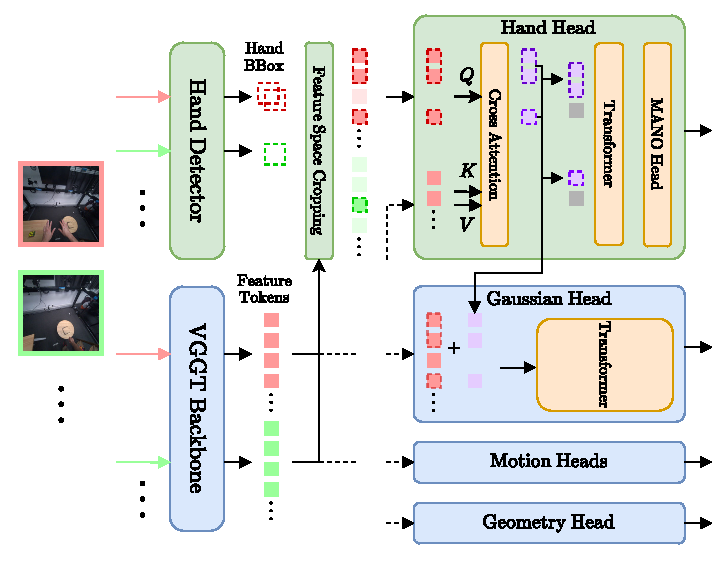
\includegraphics[width=0.70\linewidth]{figures/architecture.pdf}
  \caption{\textbf{Architecture overview.} A frozen VGGT backbone, inherited
  from NeoVerse~\cite{yang2026neoverse}, encodes the egocentric clip. We add a
  HaMeR-style~\cite{pavlakos2024hamer} hand head that regresses MANO parameters
  for both hands from feature-space crops, and we inject its intermediate
  hand-aware tokens into the Gaussian head's feature pyramid (green modules are
  added by us). The camera, Gaussian and hand heads are trained jointly while
  the backbone stays frozen.}
  \label{fig:arch}
\end{figure*}

\subsection{Overview and backbone}
\label{sec:overview}
The input is a monocular egocentric clip $\mathbf{I}\in\mathbb{R}^{T\times 3\times
H\times W}$ of $T{=}16$ frames at $H{=}W{=}224$. The frozen backbone takes RGB only
and regresses each frame's camera pose. Egocentric rigs are calibrated, so we take
the per-frame intrinsics $K_t=(f_t,c_{x,t},c_{y,t})$ as known and use them to
reproject the predicted hands into the image (\cref{sec:handhead}), not as backbone
input. Per frame $t$ the model predicts (i) a pixel-aligned
4D Gaussian field $\{(\boldsymbol{\mu}_k,\boldsymbol{\Sigma}_k,o_k,\mathbf{c}_k)\}_k$
and a depth map $D_t\in\mathbb{R}^{H\times W}$, (ii) the camera pose, and (iii) for
each visible hand $h\in\{\mathrm{L},\mathrm{R}\}$ the MANO~\cite{romero2017mano}
parameters $\mathbf{m}_{t,h}=(\mathbf{t}_{t,h},\mathbf{q}_{t,h},
\boldsymbol{\theta}_{t,h},\boldsymbol{\beta}_{t,h})\in\mathbb{R}^{32}$: a
translation $\mathbf{t}_{t,h}\in\mathbb{R}^{3}$, a global rotation
$\mathbf{q}_{t,h}\in\mathbb{R}^{4}$ (quaternion), a reduced pose
$\boldsymbol{\theta}_{t,h}\in\mathbb{R}^{15}$, and a shape
$\boldsymbol{\beta}_{t,h}\in\mathbb{R}^{10}$. We build on
NeoVerse~\cite{yang2026neoverse}, whose VGGT backbone~\cite{wang2025vggt} produces
multi-level dense features that are decoded by DPT-style heads into camera, depth
and Gaussian parameters. Each pixel emits a Gaussian (mean, covariance, opacity
and color), and a frame is rendered by differentiable alpha compositing as in
3DGS~\cite{kerbl20233d}, using the gsplat rasterizer. We keep the backbone
\emph{frozen} (no gradient flows into it) throughout, both to preserve the
geometry prior learned at scale and to keep training tractable on a single GPU.
All new capacity lives in the hand head and in the injection pathway
(\cref{fig:arch}).

\subsection{Multi-hand MANO head}
\label{sec:handhead}
MANO~\cite{romero2017mano} maps pose $\boldsymbol{\theta}$ and shape
$\boldsymbol{\beta}$ to a hand mesh by linear blend skinning,
\begin{equation}
  \mathbf{V}(\boldsymbol{\theta},\boldsymbol{\beta}) =
  W\!\big(\bar{\mathbf{T}} + B_S(\boldsymbol{\beta}) + B_P(\boldsymbol{\theta}),\;
  J(\boldsymbol{\beta}),\; \boldsymbol{\theta},\; \mathcal{W}\big),
  \label{eq:mano}
\end{equation}
with $V{=}778$ vertices $\mathbf{V}\in\mathbb{R}^{778\times3}$, where
$\bar{\mathbf{T}}$ is the template mesh, $B_S$ and $B_P$ are the shape and pose
blend shapes, $J(\boldsymbol{\beta})$ regresses joint centers, and $W$ is the
skinning function with weights $\mathcal{W}$. The $J{=}21$ joints are
$\mathbf{J}=\mathcal{R}\mathbf{V}\in\mathbb{R}^{21\times3}$ for a fixed regressor
$\mathcal{R}$. Following HaMeR~\cite{pavlakos2024hamer}, our head is a transformer
decoder that attends to backbone features and emits, for each hand $h$, the
parameters $\mathbf{m}_h=(\mathbf{t}_h,\mathbf{q}_h,\boldsymbol{\theta}_h,
\boldsymbol{\beta}_h)$, with the metric translation $\mathbf{t}_h$ placing the
joints in camera coordinates as $\mathbf{X}_h =
\mathbf{J}(\boldsymbol{\theta}_h,\boldsymbol{\beta}_h) + \mathbf{t}_h$. We
supervise them in 2D by projecting into the image with the known camera
intrinsics $K$. This differs from HaMeR, which regresses a weak-perspective crop
camera. Because our hands are placed metrically in the camera frame, we reproject
with the real intrinsics. A single decoder pass produces both hands, conditioned on
\emph{local-global fused} features: the per-hand crop tokens cross-attend to the
global scene tokens of the backbone, so each hand prediction sees the surrounding
scene and the other hand. The fusion ablation (\cref{sec:hands}) isolates this as
the dominant design choice.

\subsection{Feature-space cropping}
\label{sec:fcrop}
A hand occupies a small fraction of an egocentric frame, so processing the full
image through the head wastes computation. Rather than re-encoding a pixel crop,
we crop in \emph{feature} space: given a per-frame hand bounding box $b_h$
(rescaled by a fixed factor to add context), we pool the backbone feature map
inside $b_h$ to obtain the hand tokens that condition the decoder. This reuses
the single backbone pass already computed for the scene and avoids a second
forward over a pixel crop, which is the dominant cost in a naive HaMeR-on-crops
pipeline.

\subsection{Hand-to-Gaussian injection}
\label{sec:inject}
The hand head produces, per hand, enhanced crop tokens
$\mathbf{E}_h\in\mathbb{R}^{K\times C}$ ($C{=}1024$) that have cross-attended to
the global scene context and now carry an explicit hand prior. For each level $i$
of the Gaussian head's DPT pyramid $\mathbf{F}_i\in\mathbb{R}^{C_i\times h_i\times
w_i}$ ($C_i\in\{256,512,1024,1024\}$), a $1{\times}1$ convolution $W_i$ maps the
tokens to $C_i$ channels and we add $\mathrm{resize}_{b_h}(W_i\mathbf{E}_h)$ into
the box region $b_h$ of $\mathbf{F}_i$, for each valid hand. The Gaussian head
then reconstructs the hand region conditioned on hand location and pose, instead
of inferring it from appearance. This injection is the only path from the hand
prior to the radiance field. The GS ablation toggles it.

\subsection{Training objective}
\label{sec:loss}
The backbone is frozen. We train the camera, Gaussian and hand heads jointly with
a sum of photometric and hand terms,
\begin{equation}
  \begin{aligned}
  \mathcal{L} =\;& \underbrace{\lambda_1 \mathcal{L}_{\mathrm{L1}} + \lambda_2 \mathcal{L}_{\mathrm{LPIPS}}}_{\text{Gaussian}}
  + \underbrace{\lambda_3 \mathcal{L}_{\mathrm{MANO}} + \lambda_4\mathcal{L}_{3\mathrm{D}} + \lambda_5\mathcal{L}_{2\mathrm{D}}}_{\text{hand}} .
  \end{aligned}
  \label{eq:loss}
\end{equation}
The Gaussian terms are an $\ell_1$ photometric loss and a perceptual
LPIPS~\cite{zhang2018lpips} loss between rendered and ground-truth frames.
$\mathcal{L}_{\mathrm{MANO}}$ is an $\ell_1$ loss on the predicted parameters
$\mathbf{m}_{t,h}$ (translation, rotation, pose and shape, masked per hand).
$\mathcal{L}_{3\mathrm{D}}$ is a pelvis-aligned error on the joints
$\mathbf{J}_{t,h}$. $\mathcal{L}_{2\mathrm{D}}$ is the 2D reprojection error of the
predicted joints against the annotated keypoints. We train with clips of $16$
frames at $224{\times}224$, AdamW, bf16 autocast, and gradient accumulation.

%==============================================================
\section{Experiments}
\label{sec:exp}

\paragraph{Dataset.}
We train and evaluate on HOT3D~\cite{banerjee2024hot3d}, an egocentric
hand-object dataset captured with Project Aria. Each sequence is a first-person
recording of a person manipulating objects, with high-fidelity 3D MANO hand
annotations and calibrated camera tracks. We use $198$ sequences, sliced into
non-overlapping $16$-frame clips, and hold out sequences for validation and
test. All metrics are computed on held-out sequences.

\paragraph{Metrics.}
For Gaussian reconstruction we report PSNR, SSIM and
LPIPS~\cite{zhang2018lpips} between rendered and ground-truth frames. For hand
estimation we report Procrustes-aligned vertex and joint error (PA-MPVPE,
PA-MPJPE, in mm) and the corresponding area-under-the-curve of correct keypoints
(AUC-V, AUC-J), the standard HaMeR protocol.

\paragraph{Baselines.}
For scene reconstruction we compare against NeoVerse in two settings: the
\emph{frozen} pretrained model run on HOT3D, and a \emph{trained} variant whose
heads we finetune on HOT3D without any hand prior. Our model adds hand injection
to the trained variant, which separates the effect of the prior from that of
finetuning. For hands the controlled comparison is internal: our
retrained head \emph{without} local-global fusion versus the full head
\emph{with} fusion, plus a decoupled variant. All are trained on HOT3D under one
protocol, so only the design choice varies. We additionally list
off-the-shelf HaMeR~\cite{pavlakos2024hamer} \emph{for reference only}. It was not
trained on the HOT3D egocentric viewpoint, so the gap to it mixes domain
adaptation with architecture and is not a clean method comparison.

\subsection{Gaussian reconstruction}
\label{sec:gs}

\begin{table}[t]
  \centering
  \begin{tabular}{lccc}
    \toprule
    Method & PSNR\,$\uparrow$ & SSIM\,$\uparrow$ & LPIPS\,$\downarrow$ \\
    \midrule
    NeoVerse (frozen)  & 35.75 & 0.970 & 0.008 \\
    NeoVerse (trained) & 36.96 & \textbf{0.977} & 0.005 \\
    Hand Inj.\ (Ours)  & \textbf{37.92} & \textbf{0.977} & \textbf{0.004} \\
    \bottomrule
  \end{tabular}
  \caption{\textbf{Gaussian reconstruction on HOT3D.} Hand-feature injection on
  top of the finetuned NeoVerse baseline improves PSNR and LPIPS, with SSIM on
  par. Higher is better for PSNR/SSIM, lower for LPIPS.}
  \label{tab:gs}
\end{table}

\Cref{tab:gs} reports the scene results. Finetuning the NeoVerse heads on HOT3D
lifts PSNR from $35.75$ to $36.96$ dB. Hand injection raises it to $37.92$ dB
($+0.96$ dB over the finetuned baseline) and lowers LPIPS from $0.005$ to
$0.004$. SSIM is saturated at $0.977$ and does not move. These are
\emph{full-frame} metrics. Hands cover a small fraction of an egocentric frame,
so the static background dominates the average and understates the gain in the
region the prior acts on. Region-masked PSNR and LPIPS are required to measure it
(\cref{sec:discuss}). \Cref{fig:bars}(top) plots the gains. \Cref{fig:gsqual}
shows a reconstructed Gaussian frame.

\begin{figure}[t]
  \centering
  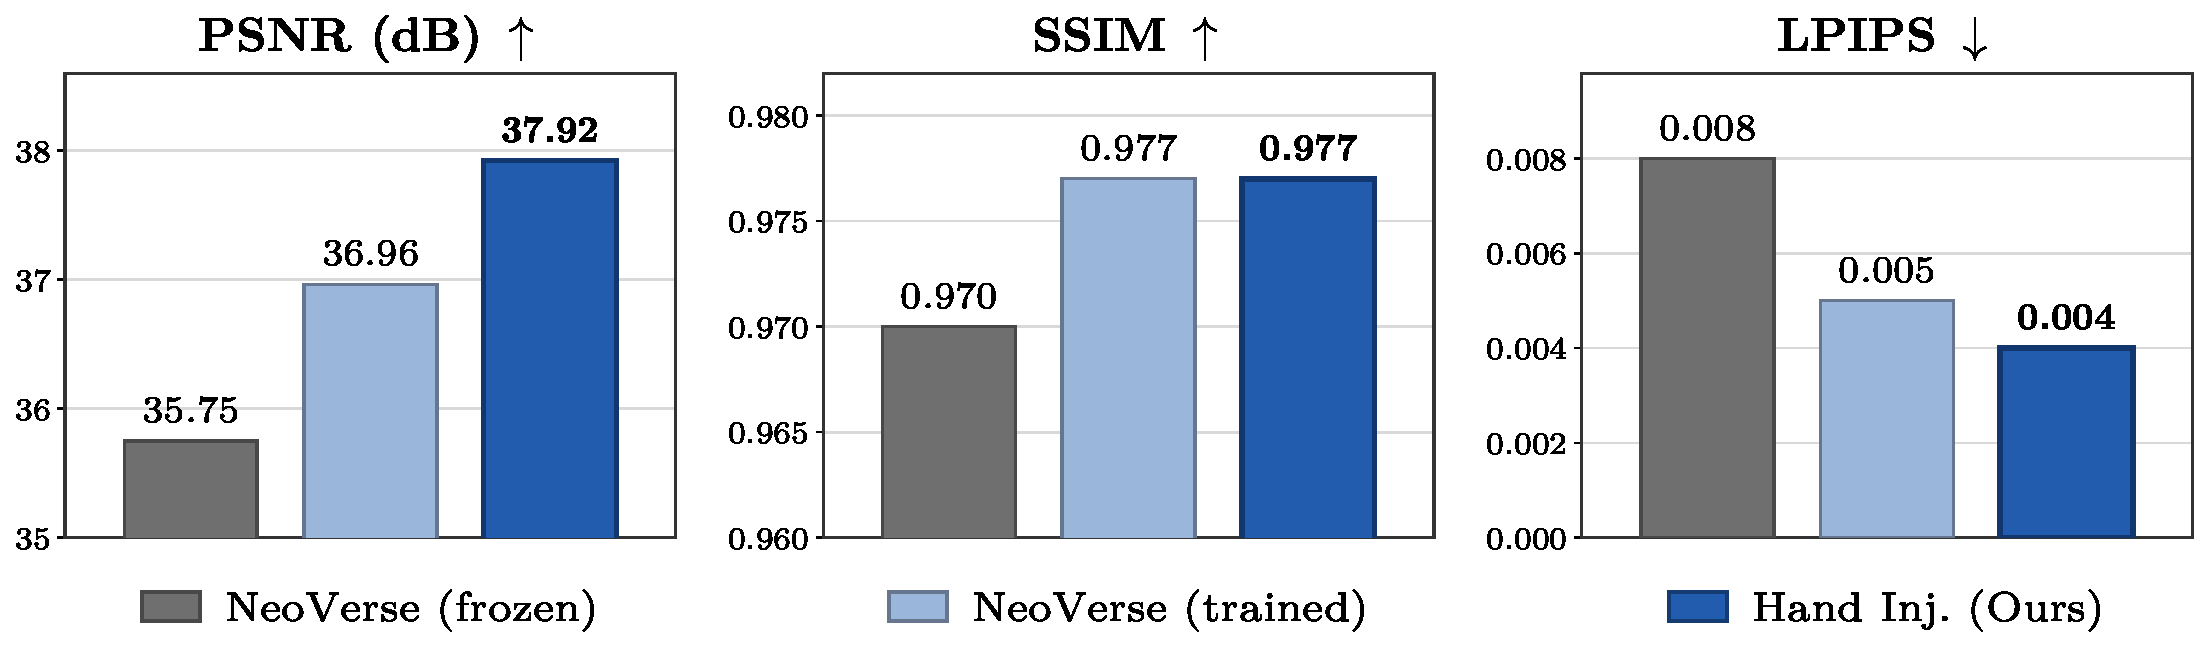
\includegraphics[width=\linewidth]{figures/gs_ablation_barchart.pdf}\\[0.4em]
  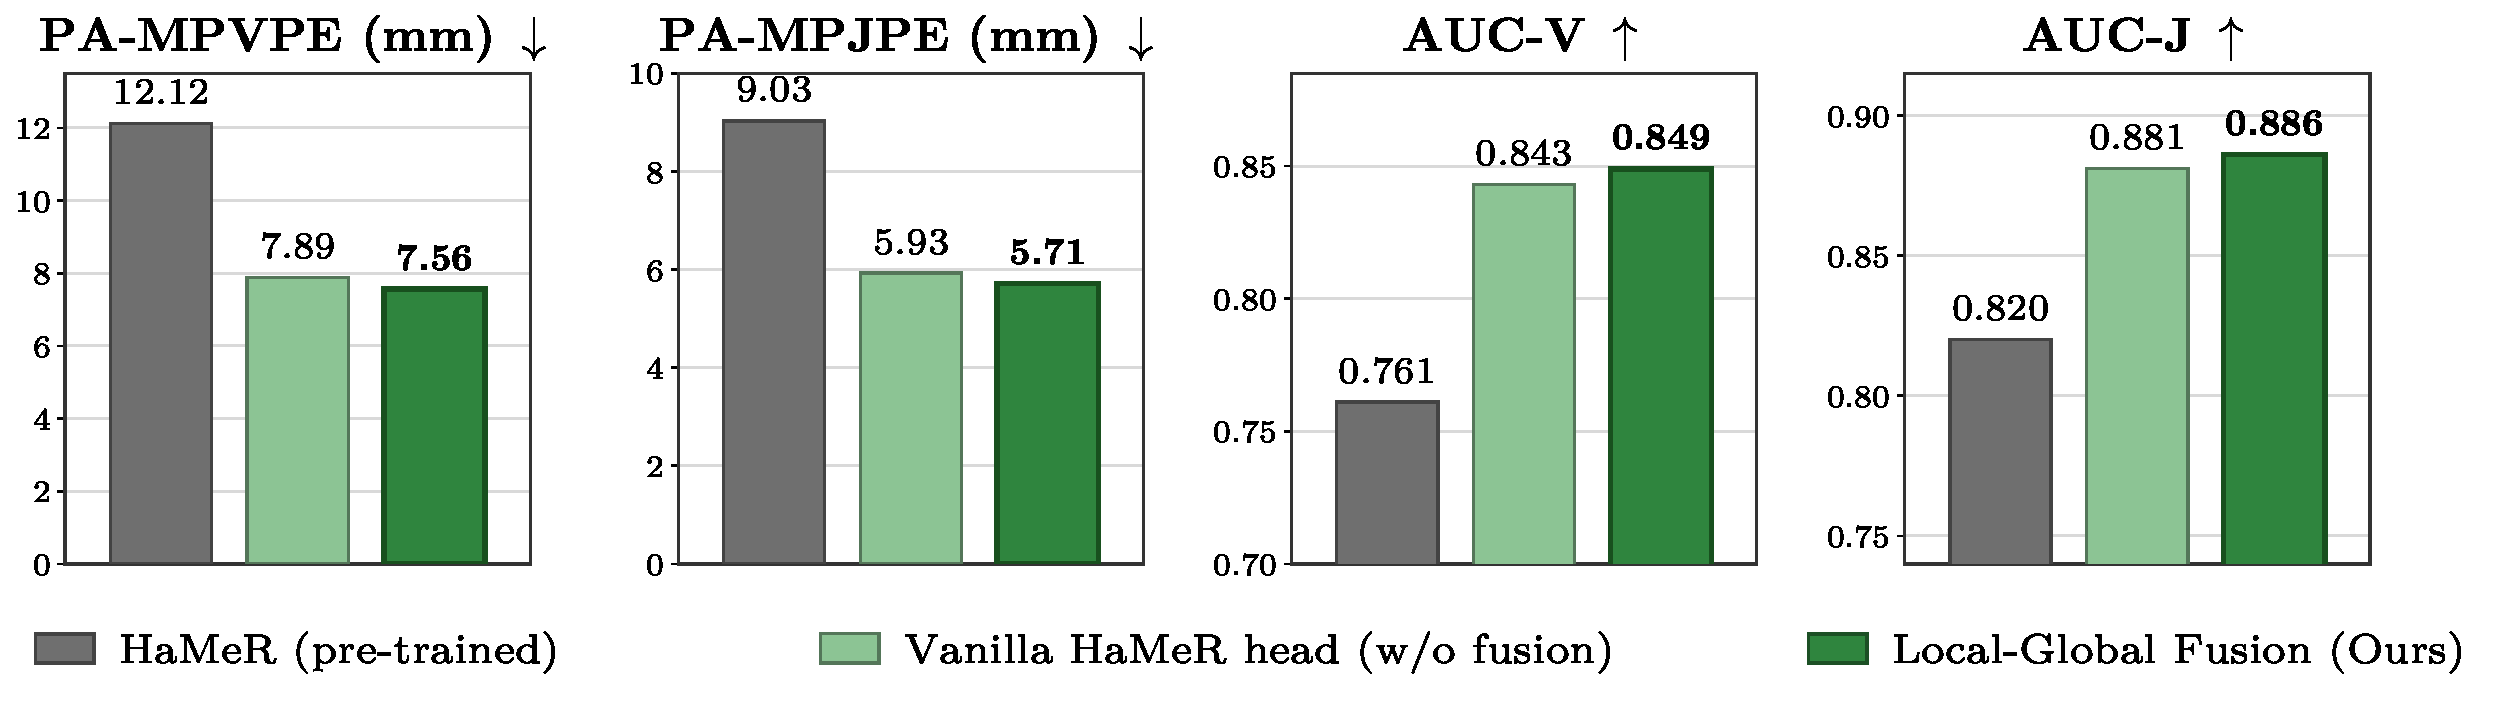
\includegraphics[width=\linewidth]{figures/hand_metrics_barchart.pdf}
  \caption{\textbf{Ablations.} Top: Gaussian reconstruction. Hand injection
  improves PSNR and LPIPS over the frozen and finetuned NeoVerse baselines.
  Bottom: hand head. Local-global fusion (cross-attention between hand crops and
  global scene features) gives the best hand-mesh accuracy and far surpasses
  off-the-shelf HaMeR.}
  \label{fig:bars}
\end{figure}

\subsection{Hand reconstruction}
\label{sec:hands}

\begin{table}[t]
  \centering
  \setlength{\tabcolsep}{4pt}
  \resizebox{\linewidth}{!}{%
  \begin{tabular}{lcccc}
    \toprule
    Method & \makecell{PA-MPVPE\\$\downarrow$} & \makecell{PA-MPJPE\\$\downarrow$}
           & \makecell{AUC-V\\$\uparrow$} & \makecell{AUC-J\\$\uparrow$} \\
    \midrule
    HaMeR (pre-trained, \emph{reference}) & 12.12 & 9.03 & 0.761 & 0.820 \\
    \midrule
    Ours, head w/o fusion     & 7.89  & 5.93 & 0.843 & 0.881 \\
    Ours, local-global fusion & \textbf{7.56} & \textbf{5.71} & \textbf{0.849} & \textbf{0.886} \\
    \bottomrule
  \end{tabular}}
  \caption{\textbf{Hand reconstruction on HOT3D} (PA-MPVPE / PA-MPJPE in mm). Our
  controlled result is the fusion ablation (bottom two rows, identical protocol):
  local-global fusion improves every metric. Off-the-shelf HaMeR is listed for
  reference only and is not trained on the HOT3D viewpoint, so its gap conflates
  domain adaptation with architecture.}
  \label{tab:hand}
\end{table}

\Cref{tab:hand} reports the hand results. The main comparison is the fusion
ablation, with the same training protocol in both rows. Local-global fusion
lowers PA-MPJPE from $5.93$ to $5.71$ mm and improves the other three metrics. A
variant that detaches the hand tokens from the scene gradient is worse on all
four metrics, so the gain comes from coupling the hand to the scene. We list
off-the-shelf HaMeR ($9.03$ mm PA-MPJPE) as a reference. It was not trained on the
HOT3D viewpoint, so this gap also reflects in-domain training, and we do not read
it as a method result. \Cref{fig:handqual} shows example fits and projected
joints.

\begin{figure}[t]
  \centering
  \begin{tabular}{@{}c@{\hspace{0.04\linewidth}}c@{}}
    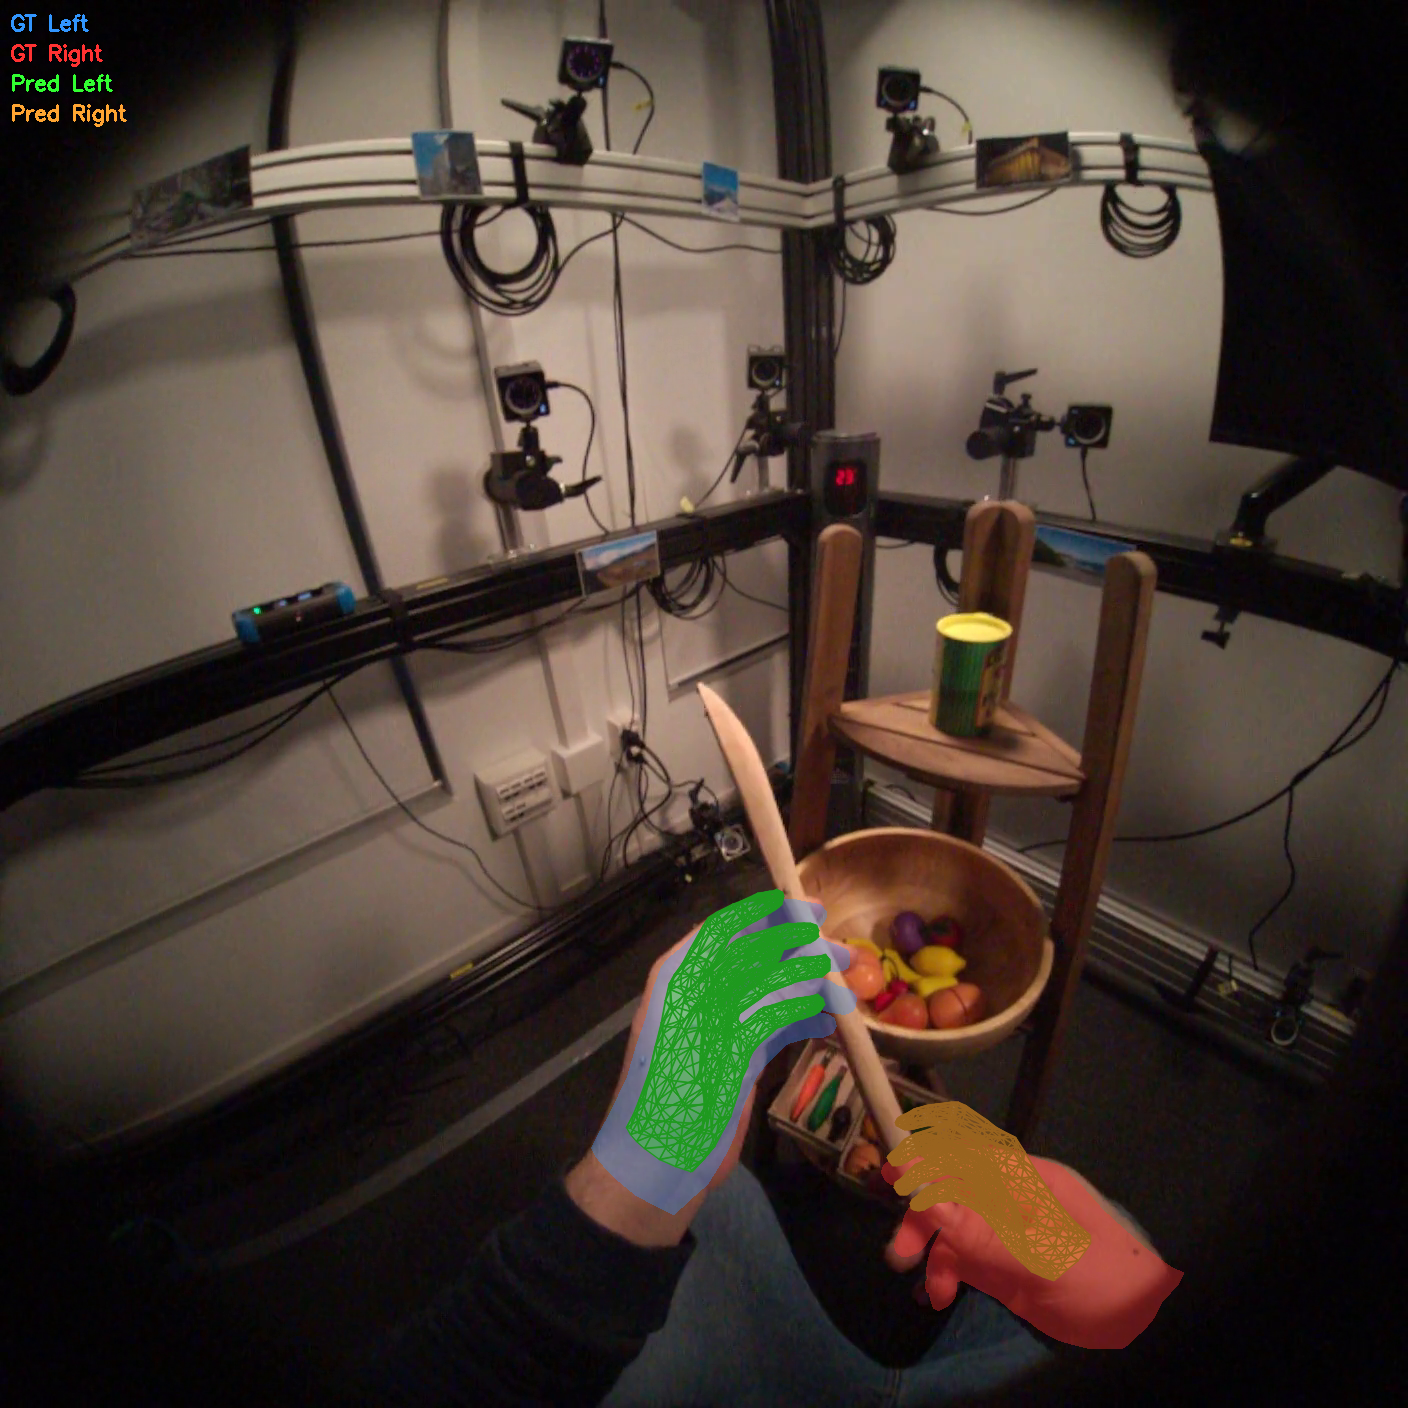
\includegraphics[width=0.47\linewidth]{figures/3d_viz.png} &
    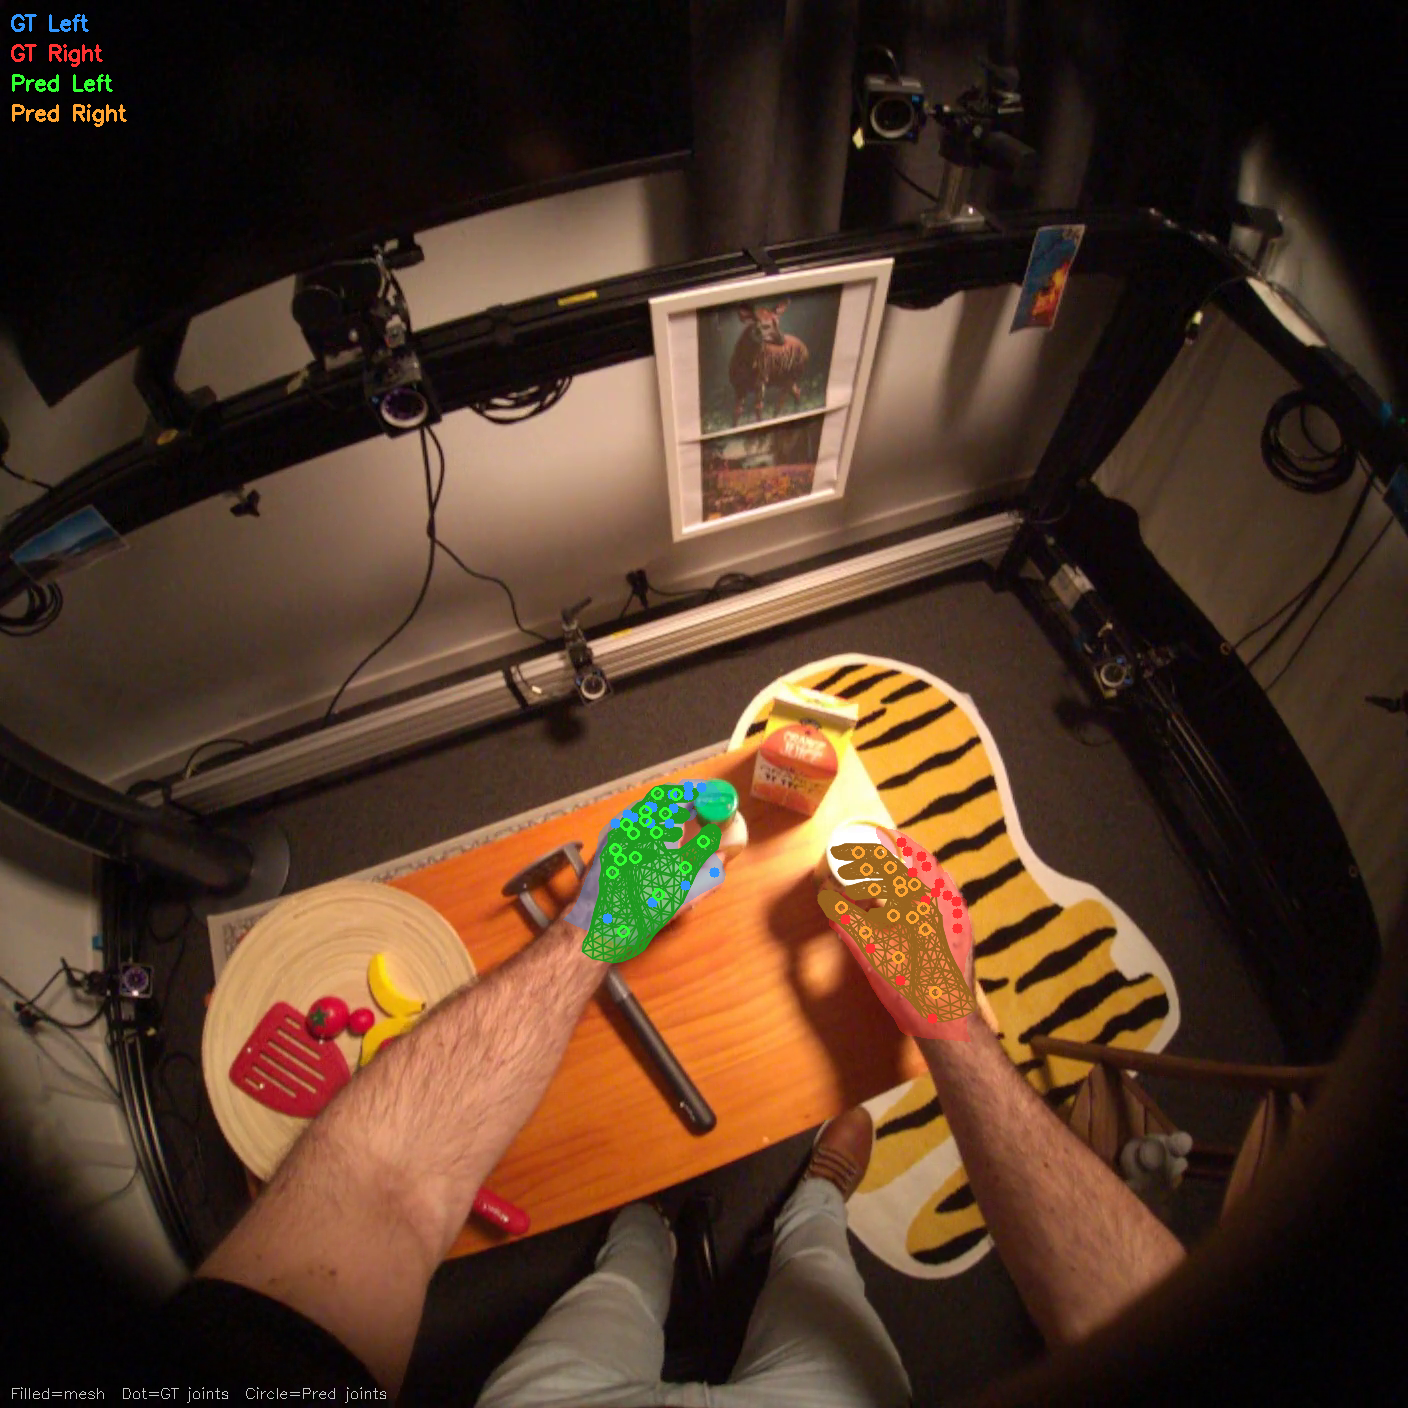
\includegraphics[width=0.47\linewidth]{figures/2d_viz.png} \\
    {\small (a) 3D hand mesh} & {\small (b) projected joints} \\
  \end{tabular}
  \caption{\textbf{Hand predictions vs.\ ground truth.} (a) the recovered 3D
  MANO mesh. (b) the same prediction with 3D joints projected into the image.}
  \label{fig:handqual}
\end{figure}

\begin{figure}[t]
  \centering
  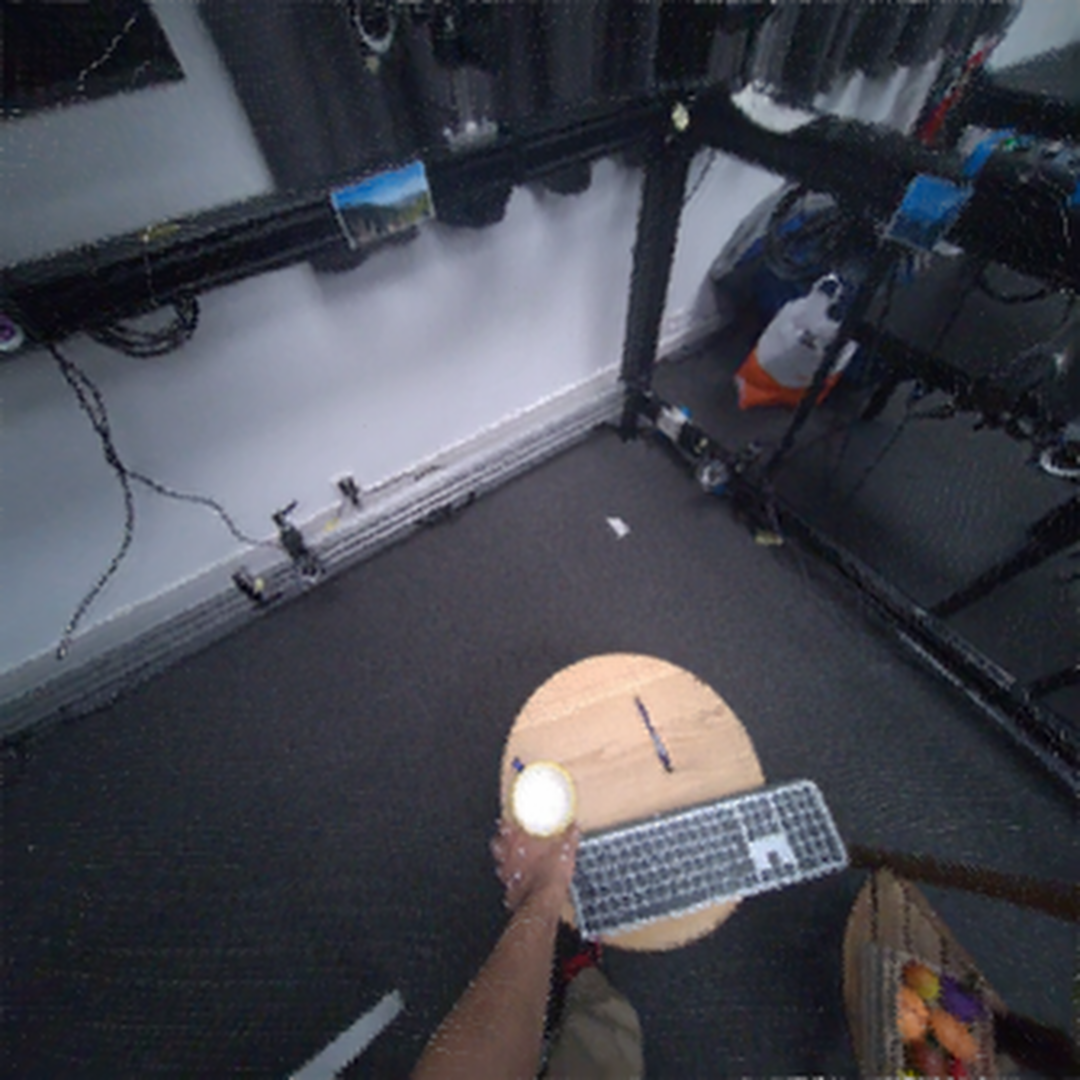
\includegraphics[width=0.72\linewidth]{figures/gs_recon.png}
  \caption{\textbf{Gaussian head, qualitative.} A reconstructed Gaussian frame on
  HOT3D.}
  \label{fig:gsqual}
\end{figure}

\subsection{Discussion}
\label{sec:discuss}
We make two observations. First, the hand prior improves the scene reconstruction
itself: full-frame PSNR and LPIPS rise while SSIM stays flat. Second, the hand
accuracy comes from fusing local hand crops with global scene context, since the
decoupled variant is worse. Both support the hypothesis that a parametric hand
estimate is a cheap and useful prior for egocentric 4D reconstruction.

\paragraph{Next measurement.}
The scene gains above are full-frame and therefore diluted, since the background
dominates the average while the prior acts on the hand and object regions. The
next experiment is to recompute PSNR and LPIPS inside masks of those regions. The
pipeline already caches the projected MANO joints and hand boxes, and HOT3D
provides object poses and meshes for the object masks. We expect a larger gain in
the masked regions. An improvement in the object region would be the stronger
result, since it shows that the hand prior helps reconstruct the manipulated
object. We report this as the main open direction, not a completed result.

\paragraph{Other limitations.}
We keep the backbone frozen, which bounds domain adaptation. Parameter-efficient
finetuning is a natural extension. Our hand comparison is controlled only
internally (the fusion ablation), and a fair external baseline would finetune
HaMeR or a similar model in-domain under our protocol. Finally, all results are on
HOT3D. Transfer to a second dataset such as ARCTIC~\cite{fan2023arctic} or
EPIC-KITCHENS~\cite{damen2018epic} would test whether the effect is dataset
specific. We also report single-run numbers without variance, which per-sequence
statistics should accompany.

%==============================================================
\section{Contributions, Work Distribution and Code Provenance}
\label{sec:contrib}

\paragraph{Novel contributions.}
We report two main results. First, a hand prior injected into a feedforward 4D
Gaussian head improves the scene reconstruction, not only the hand mesh. Second,
the hand accuracy comes from local-global fusion, as the decoupled variant shows.
The mechanism is a multi-hand single-pass MANO head on a frozen VGGT/NeoVerse
backbone, feature-space cropping, and hand-to-Gaussian injection into the DPT
pyramid. To our knowledge this combination has not been used before. The
concurrent Hand3R~\cite{hu2026hand3r} also reconstructs hands and
scene, but fuses two reconstructed geometries online, while we inject a hand prior
into a feedforward Gaussian head and supervise it with photometric reconstruction.

\paragraph{Work distribution.}
The project was carried out by three team members. \textbf{Dario Monopoli} led
the data pipeline (HOT3D loading, MANO ground-truth caching, hand bounding-box
extraction), the training and evaluation infrastructure, and the performance and
profiling work that made full-dataset training feasible. \textbf{Batuhan Iliev}
led the hand head (the multi-hand MANO transformer decoder and the local-global
fusion) and the hand-metric evaluation. \textbf{Marian Schneider} led the
hand-to-Gaussian injection and the Gaussian reconstruction evaluation. Method
design, the ablation study, the report and the
poster were shared across all three. (Team members should adjust this paragraph
to match their own records.)

\paragraph{Code we used vs.\ code we wrote.}
We \emph{reused} external code and models: the NeoVerse 4D world model and VGGT
backbone~\cite{yang2026neoverse,wang2025vggt} with its frozen pretrained weights,
the MANO hand model~\cite{romero2017mano}, the HaMeR architecture as the starting
point for our head~\cite{pavlakos2024hamer}, the differentiable Gaussian
rasterizer of the backbone, and standard LPIPS and rendering-metric
implementations. We \emph{implemented ourselves} the multi-hand MANO head and its
local-global fusion, the feature-space cropping, the hand-to-Gaussian injection
into the DPT pyramid, the HOT3D data pipeline and caching, the training loop and
loss (\cref{eq:loss}), and the evaluation and ablation harness for \cref{tab:gs}
and \cref{tab:hand}.

%==============================================================
\section{Conclusion}
\label{sec:conclusion}
We presented a feedforward 4D Gaussian model for egocentric video with a hand
head. We attach a multi-hand MANO head to a frozen VGGT/NeoVerse backbone and
inject its features into the Gaussian head. On HOT3D the hand prior raises
full-frame scene PSNR from $36.96$ to $37.92$ dB over the finetuned baseline.
Local-global fusion lowers hand error from $5.93$ to $5.71$ mm PA-MPJPE, and the
decoupled variant is worse. Feature-space cropping keeps the added cost low.
Region-masked evaluation of the hand and object regions is the next step toward a
conclusive result.

{
    \small
    \bibliographystyle{ieeenat_fullname}
    \bibliography{references}
}

\end{document}
